% ============================================================
%  TD N°07 — Naive Bayes & Raisonnement Bayésien
%  Compte Rendu Académique
%  Auteur : Chabbaki Ayman — MDSBDIA26 — Groupe G1
% ============================================================
\documentclass[12pt,a4paper]{article}

\usepackage[utf8]{inputenc}
\usepackage[T1]{fontenc}
\usepackage[french]{babel}
\usepackage[top=2.5cm, bottom=2.5cm, left=2.5cm, right=2.5cm]{geometry}
\usepackage{fancyhdr}
\usepackage{titlesec}
\usepackage{parskip}
\usepackage{lmodern}
\usepackage{microtype}
\usepackage[dvipsnames,table]{xcolor}
\usepackage{graphicx}
\usepackage{float}
\usepackage{tikz}
\usepackage{amsmath,amssymb}
\usepackage{bm}
\usepackage{booktabs}
\usepackage{tabularx}
\usepackage{array}
\usepackage{colortbl}
\usepackage{multirow}
\usepackage[most]{tcolorbox}
\tcbuselibrary{breakable, skins}
\usepackage{hyperref}
\hypersetup{colorlinks=true, linkcolor=darkblue, urlcolor=tealcolor}
\usepackage{enumitem}

% ─── Palette ────────────────────────────────────────────────
\definecolor{darkblue}{RGB}{26,37,80}
\definecolor{tealcolor}{RGB}{26,122,110}
\definecolor{crimson}{RGB}{156,61,56}
\definecolor{amber}{RGB}{176,125,58}
\definecolor{bayespurple}{RGB}{80,50,130}
\definecolor{lightgray}{RGB}{245,245,245}
\definecolor{midgray}{RGB}{180,180,180}

% ─── Titres ─────────────────────────────────────────────────
\titleformat{\section}{\large\bfseries\color{darkblue}}{\thesection.}{.5em}{}
  [\color{tealcolor}\rule{\linewidth}{0.6pt}]
\titleformat{\subsection}{\normalsize\bfseries\color{tealcolor}}{\thesubsection}{.5em}{}
\titleformat{\subsubsection}{\small\bfseries\color{amber}}{\thesubsubsection}{.5em}{}

% ─── En-tête / Pied ─────────────────────────────────────────
\pagestyle{fancy}\fancyhf{}
\fancyhead[L]{\small\color{darkblue}\bfseries TD 7 — Naive Bayes \& Raisonnement Bayésien}
\fancyhead[R]{\small\color{darkblue} Chabbaki Ayman · MDSBDIA26 · G1}
\fancyfoot[C]{\small\color{midgray}--- \thepage\ ---}
\renewcommand{\headrulewidth}{0.4pt}
\renewcommand{\headrule}{\hbox to\headwidth{\color{darkblue}\leaders\hrule height\headrulewidth\hfill}}

% ─── tcolorbox ──────────────────────────────────────────────
\tcbset{base/.style={breakable,enhanced,fonttitle=\bfseries\small,
  left=6pt,right=6pt,top=5pt,bottom=5pt,boxrule=0.5pt}}

\newtcolorbox{reponsebox}[1][]{base,colback=tealcolor!8,colframe=tealcolor,
  coltitle=white,colbacktitle=tealcolor,title={Réponse},#1}
\newtcolorbox{resultbox}[1][]{base,colback=darkblue!6,colframe=darkblue,
  coltitle=white,colbacktitle=darkblue,title={Résultat expérimental},#1}
\newtcolorbox{observbox}[1][]{base,colback=amber!8,colframe=amber,
  coltitle=white,colbacktitle=amber,title={Observation clé},#1}
\newtcolorbox{theorbox}[1][]{base,colback=bayespurple!6,colframe=bayespurple,
  coltitle=white,colbacktitle=bayespurple,title={Théorie Bayésienne},#1}

% ============================================================
\begin{document}
% ============================================================

% ─── Page de titre ──────────────────────────────────────────
\begin{titlepage}
\begin{tikzpicture}[remember picture,overlay]
  \fill[darkblue] (current page.north west) rectangle ([yshift=-4.5cm]current page.north east);
  \fill[tealcolor] ([yshift=-4.5cm]current page.north west) rectangle ([yshift=-5.1cm]current page.north east);
  \fill[bayespurple] ([yshift=-5.1cm]current page.north west) rectangle ([yshift=-5.4cm]current page.north east);
\end{tikzpicture}

\vspace*{2.5cm}
{\color{white}\raggedright
  \hspace{1cm}{\fontsize{11}{13}\selectfont Master Intelligence Artificielle}\par
  \hspace{1cm}{\fontsize{10}{12}\selectfont Machine Learning — Semestre 2024–2025}\par
  \vspace{0.6cm}
  \hspace{1cm}{\fontsize{9}{11}\selectfont\color{white!80!darkblue} Pr. BEN LAHMAR EL Habib}
}
\vspace{3.5cm}
\begin{center}
  \begin{tcolorbox}[enhanced,width=0.88\textwidth,colback=white,colframe=darkblue,
    boxrule=2pt,arc=4pt,drop shadow={darkblue!40}]
    \centering\vspace{0.4cm}
    {\color{bayespurple}\fontsize{10}{12}\selectfont\bfseries TRAVAUX DIRIGÉS N°\,07}\\[0.4cm]
    {\color{darkblue}\fontsize{18}{22}\selectfont\bfseries Naive Bayes}\\[0.2cm]
    {\color{darkblue}\fontsize{13}{16}\selectfont\bfseries \& Raisonnement Bayésien}\\[0.3cm]
    {\color{tealcolor}\fontsize{10}{12}\selectfont\itshape
      Théorème de Bayes · Lissage de Laplace · GaussianNB · MultinomialNB · Calibration}\\[0.3cm]
    \color{midgray}\rule{0.7\linewidth}{0.5pt}\\[0.3cm]
    {\fontsize{11}{13}\selectfont\bfseries Chabbaki Ayman}\\[0.1cm]
    {\color{tealcolor}\fontsize{10}{12}\selectfont MDSBDIA26 — Groupe G1}\\[0.3cm]\vspace{0.2cm}
  \end{tcolorbox}
\end{center}
\vfill
\begin{center}
\begin{tabular}{ccc}
  \textcolor{darkblue}{\textbf{Datasets}} & \quad & \textcolor{darkblue}{\textbf{Outils}} \\
  \textcolor{tealcolor}{Météo · BankChurners · SMS Spam} & & \textcolor{tealcolor}{sklearn · numpy · pandas} \\[1em]
  \textcolor{darkblue}{\textbf{Modèles}} & & \textcolor{darkblue}{\textbf{Date}} \\
  \textcolor{tealcolor}{GaussianNB · BernoulliNB · MultinomialNB} & & \textcolor{tealcolor}{Juin 2026}
\end{tabular}
\end{center}
\end{titlepage}

\tableofcontents\newpage

% ============================================================
\section{Introduction — Fondements du Raisonnement Bayésien}
% ============================================================

\begin{theorbox}
\textbf{Théorème de Bayes :}
$$P(C|\mathbf{X}) = \frac{P(\mathbf{X}|C) \cdot P(C)}{P(\mathbf{X})} \qquad
\text{avec } P(\mathbf{X}) = \sum_c P(\mathbf{X}|c) \cdot P(c)$$

\textbf{Hypothèse naïve :} $P(\mathbf{X}|C) = \prod_i P(x_i|C)$ — indépendance conditionnelle

\textbf{Décision :} $\hat{y} = \arg\max_c P(C=c) \cdot \prod_i P(x_i|C=c)$ — en log-espace pour stabilité numérique

\textbf{Lissage de Laplace :} $P(x_i|C) = \dfrac{N(x_i,C) + \alpha}{N(C) + \alpha \cdot |V|}$
— évite les probabilités nulles catastrophiques ($\alpha=1$ par défaut)
\end{theorbox}

Naive Bayes est souvent le \textbf{premier algorithme probabiliste} présenté : simple ($O(n \cdot d)$ entraînement), rapide, interpretable. Ce TD en explore toutes les facettes sur le dataset \textbf{BankChurners} (10\,127 clients, 19 features, 16{,}07\% de churn) et un exemple météo du cours (14 jours).

% ============================================================
\section{Partie 1 — Calcul Manuel avec le Théorème de Bayes}
% ============================================================

\subsection{Q1.1 — Dataset Météo : Bayes From Scratch}

\begin{resultbox}
\textbf{Dataset météo (14 jours) — Probabilités a priori :}
\[
P(\text{Jouer=Oui}) = \frac{9}{14} = 0{,}6429 \qquad P(\text{Jouer=Non}) = \frac{5}{14} = 0{,}3571
\]

\textbf{Nouveau jour : Ensoleillé, Frais, Normale, Vent=Oui}
\begin{center}
\small
\begin{tabular}{lcccc}
\toprule
\textbf{Classe} & $P(\text{Ciel}=\text{Ens.}|\cdot)$ & $P(\text{Temp}=\text{Frais}|\cdot)$ & $P(\text{Hum}=\text{Norm.}|\cdot)$ & $P(\text{Vent=Oui}|\cdot)$ \\
\midrule
Jouer=Oui & $2/9 = 0{,}222$ & $3/9 = 0{,}333$ & $6/9 = 0{,}667$ & $3/9 = 0{,}333$ \\
Jouer=Non & $3/5 = 0{,}600$ & $1/5 = 0{,}200$ & $1/5 = 0{,}200$ & $3/5 = 0{,}600$ \\
\bottomrule
\end{tabular}
\end{center}

\textbf{Scores (log-espace) :} $\text{log-score}(\text{Oui}) = -4{,}5486$ \quad $\text{log-score}(\text{Non}) = -5{,}2701$

\textbf{Prédiction : Jouer = \textcolor{tealcolor}{Oui}}
\end{resultbox}

\begin{reponsebox}
\textbf{Q1 — Vérification manuelle :}
\begin{align*}
P(\text{Oui}|\mathbf{X}) &\propto \tfrac{9}{14} \times \tfrac{2}{9} \times \tfrac{3}{9} \times \tfrac{6}{9} \times \tfrac{3}{9} = 0{,}00529\\
P(\text{Non}|\mathbf{X}) &\propto \tfrac{5}{14} \times \tfrac{3}{5} \times \tfrac{1}{5} \times \tfrac{1}{5} \times \tfrac{3}{5} = 0{,}00514
\end{align*}

\textbf{Q2 — Classe gagnante :} La classe \textbf{Oui} l'emporte de justesse ($0{,}00529 > 0{,}00514$). La probabilité a posteriori normalisée est $P(\text{Oui}|\mathbf{X}) \approx 0{,}507$ — une décision très marginale. Cela illustre l'importance du prior : sans le terme $P(C)$, la décision pourrait s'inverser.

\textbf{Q3 — Cas Nuageux, Chaud, Élevée, Oui — Problème zéro :} On cherche $P(\text{Ciel=Nuageux} | \text{Jouer=Non})$ : dans les 5 jours Non, aucun n'est Nuageux → $P=0$ → le produit entier vaut 0. Une seule valeur absente en entraînement rend le modèle inutilisable — c'est le défaut fondamental que Laplace résout.
\end{reponsebox}

\subsection{Q1.2 — Lissage de Laplace}

\begin{resultbox}
\textbf{Cas problématique : Nuageux, Chaud, Élevée, Vent=Oui}

$P(\text{Ciel=Nuageux} | \text{Jouer=Non}) = 0/5 = 0$ → log-score $= -\infty$
\begin{center}
\begin{tabular}{cccl}
\toprule
$\alpha$ & Score Oui & Score Non & Prédiction \\
\midrule
0{,}1 & $-4{,}9245$ & $-6{,}6806$ & \textbf{Oui} \\
1{,}0 & $-4{,}7268$ & $-4{,}9860$ & \textbf{Oui} \\
5{,}0 & $-4{,}3848$ & $-4{,}6052$ & \textbf{Oui} \\
100{,}0 & converge & vers prior & \textbf{Oui} (priorité prior) \\
\bottomrule
\end{tabular}
\end{center}
Avec $\alpha=1$ : $P(\text{Nuageux}|\text{Non}) = \frac{0+1}{5+1\times3} = \frac{1}{8} = 0{,}125 > 0$
\end{resultbox}

\begin{reponsebox}
\textbf{Q4 — Sans lissage :} $P(\text{Nuageux}|\text{Non})=0$ → log-score Non $= -\infty$. Le modèle ne peut pas prédire — une seule vraisemblance nulle détruit toute l'information des autres features, quelle que soit leur contribution individuelle.

\textbf{Q5 — Avec $\alpha=1$ :} La prédiction reste \textbf{Oui}. Le lissage affecte légèrement toutes les probabilités (en ajoutant $\alpha$ au numérateur et $\alpha\cdot|V|$ au dénominateur), mais l'impact est faible pour les valeurs bien représentées.

\textbf{Q6 — Grand $\alpha$ (100) :} Toutes les probabilités convergent vers l'uniforme $1/|V|$ — le modèle ignore les données et prédit la classe majoritaire (Oui, 9/14). C'est le régime de \textbf{biais maximal, variance nulle} : aucune information discriminante n'est exploitée.
\end{reponsebox}

% ============================================================
\section{Partie 2 — Les Trois Variantes Sklearn}
% ============================================================

\subsection{Q2.1 — GaussianNB sur BankChurners}

\begin{resultbox}
\textbf{GaussianNB — BankChurners (8101 train / 2026 test)}
\begin{center}
\begin{tabular}{lcccc}
\toprule
\textbf{Classe} & \textbf{Précision} & \textbf{Rappel} & \textbf{F1-score} & \textbf{Support} \\
\midrule
Existing (0) & 0{,}91 & 0{,}95 & 0{,}93 & 1\,701 \\
Attrited (1) & 0{,}67 & 0{,}53 & \textbf{0{,}59} & 325 \\
\midrule
Accuracy & \multicolumn{4}{c}{0{,}88} \\
\midrule
\textbf{AUC-ROC} & \multicolumn{4}{c}{\textbf{0{,}8400}} \\
\textbf{F1 churn} & \multicolumn{4}{c}{0{,}5921} \\
\bottomrule
\end{tabular}
\end{center}

\textbf{Probabilités a priori apprises :} $P(\text{Existing})=0{,}8393$, $P(\text{Attrited})=0{,}1607$

\textbf{Moyennes par classe (top features) :}
\begin{center}
\begin{tabular}{lccc}
\toprule
\textbf{Feature} & \textbf{$\mu$ Existing} & \textbf{$\mu$ Attrited} & \textbf{Différence} \\
\midrule
Total\_Trans\_Ct & 68{,}55 & 44{,}61 & $-23{,}94$ $(-35\%)$ \\
Total\_Revolving\_Bal & 1263{,}07 & 669{,}50 & $-593{,}58$ $(-47\%)$ \\
Total\_Trans\_Amt & 4645{,}96 & 3041{,}37 & $-1604{,}59$ $(-35\%)$ \\
Months\_Inactive\_12\_mon & 2{,}28 & 2{,}71 & $+0{,}43$ $\uparrow$ \\
Contacts\_Count\_12\_mon & 2{,}36 & 2{,}98 & $+0{,}62$ $\uparrow$ \\
\bottomrule
\end{tabular}
\end{center}
\end{resultbox}

\begin{figure}[H]
  \centering
  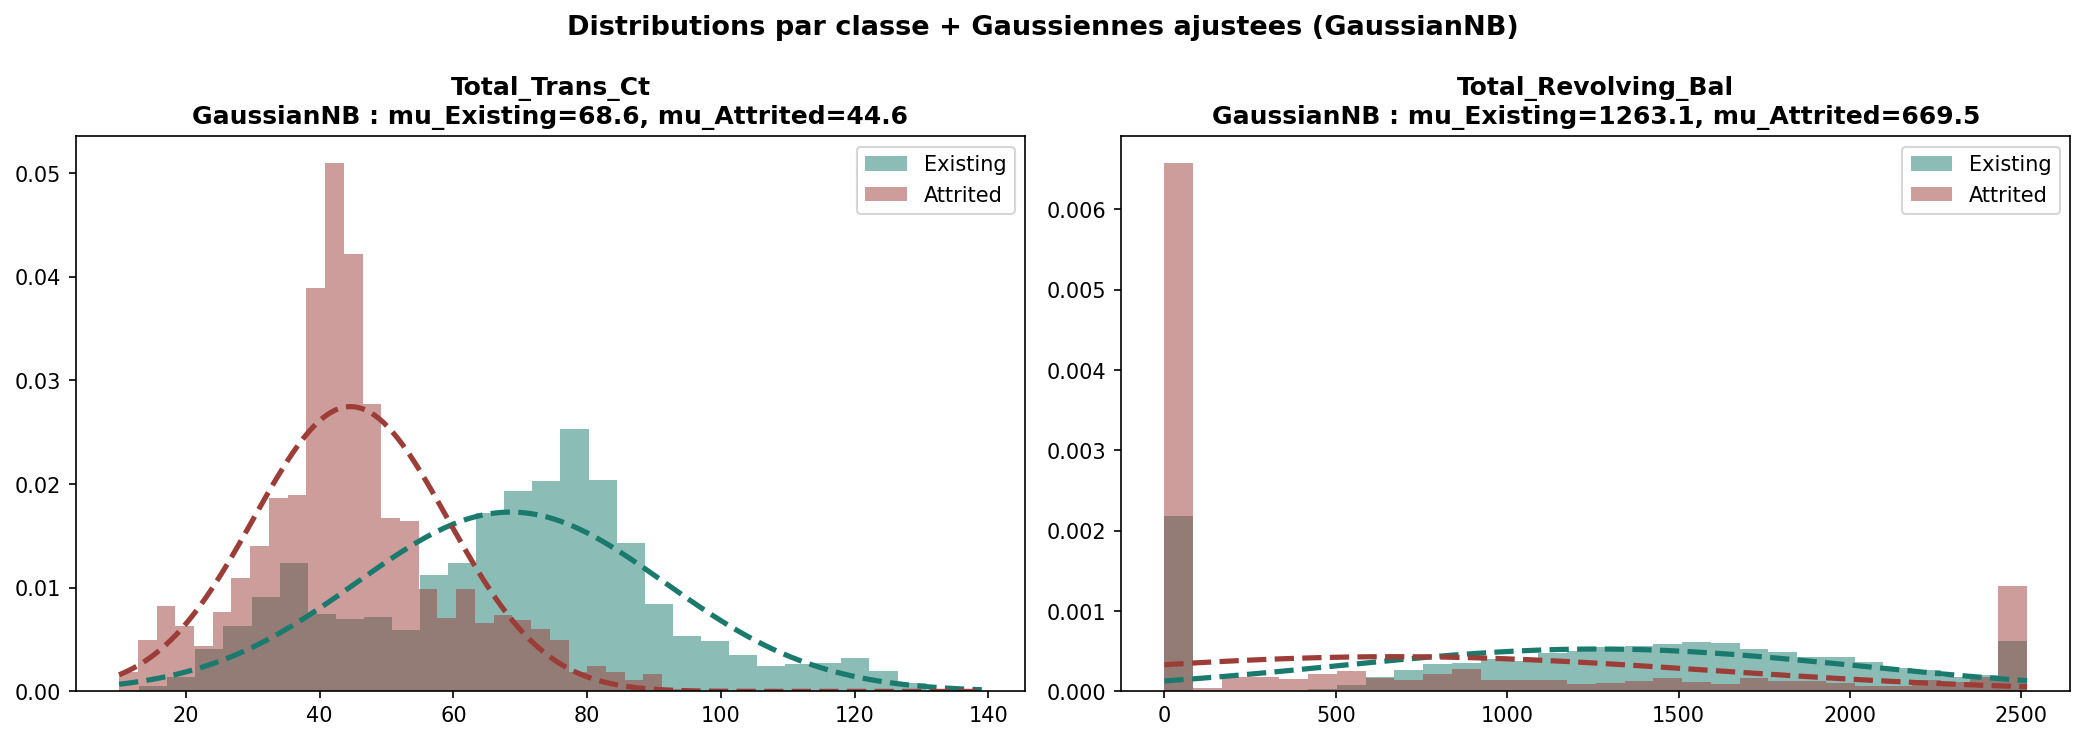
\includegraphics[width=\textwidth]{fig_gnb_distributions.png}
  \caption{Distributions par classe et gaussiennes ajustées par GaussianNB pour \texttt{Total\_Trans\_Ct} et \texttt{Total\_Revolving\_Bal}. Les distributions réelles sont asymétriques ou bimodales — l'hypothèse gaussienne est approximative.}
  \label{fig:gnb_dist}
\end{figure}

\begin{reponsebox}
\textbf{Q7 — Feature la plus discriminante :}
\texttt{Total\_Revolving\_Bal} présente la plus grande différence relative ($-47\%$ entre Attrited et Existing). \texttt{Total\_Trans\_Ct} a la différence absolue la plus large ($-23{,}94$). Ces écarts sont cohérents avec l'EDA (TD3) : les clients sur le départ font moins de transactions et ont un solde revolving plus faible, indicateurs d'un désengagement progressif.

\textbf{Q8 — Ajustement des gaussiennes :}
Pour \texttt{Total\_Trans\_Ct}, la distribution est bimodale — la gaussienne ne capture pas ce pattern. Pour \texttt{Total\_Revolving\_Bal}, le pic à 0 (clients sans crédit revolving) crée une asymétrie forte. Ces violations de l'hypothèse gaussienne expliquent les limites de GaussianNB sur BankChurners.

\textbf{Q9 — AUC-ROC = 0{,}8400 :}
C'est inférieur à la Régression Logistique (0{,}9042) et au SVM (0{,}9466). GaussianNB discrimine moins bien car ses hypothèses de distributions sont violées. Il reste néanmoins un \textbf{excellent point de départ} — rapide à entraîner ($< 0{,}1$s) et sans hyperparamètres à régler.
\end{reponsebox}

\subsection{Q2.2 — BernoulliNB — Features Binaires}

\begin{resultbox}
\textbf{Features binaires créées par seuillage à la médiane (9 features)} \\
BernoulliNB ($\alpha=1$) sur BankChurners :
\begin{center}
\begin{tabular}{lccc}
\toprule
\textbf{Modèle} & \textbf{F1 Existing} & \textbf{F1 Attrited} & \textbf{Accuracy} \\
\midrule
BernoulliNB (binaire) & 0{,}90 & 0{,}36 & 0{,}82 \\
GaussianNB (continu)  & 0{,}93 & \textbf{0{,}59} & 0{,}88 \\
\bottomrule
\end{tabular}
\end{center}

\textbf{Features binaires les plus discriminantes (P(feature=1|classe)) :}
\begin{center}
\begin{tabular}{lccc}
\toprule
\textbf{Feature} & \textbf{P(·=1|Existing)} & \textbf{P(·=1|Attrited)} & \textbf{Différence} \\
\midrule
Contacts\_Count\_12\_mon\_bin & 0{,}459 & 0{,}684 & $+0{,}225$ \\
Months\_Inactive\_12\_mon\_bin & 0{,}419 & 0{,}630 & $+0{,}211$ \\
Total\_Trans\_Ct\_bin & 0{,}542 & 0{,}286 & $-0{,}256$ \\
\bottomrule
\end{tabular}
\end{center}
\end{resultbox}

\begin{figure}[H]
  \centering
  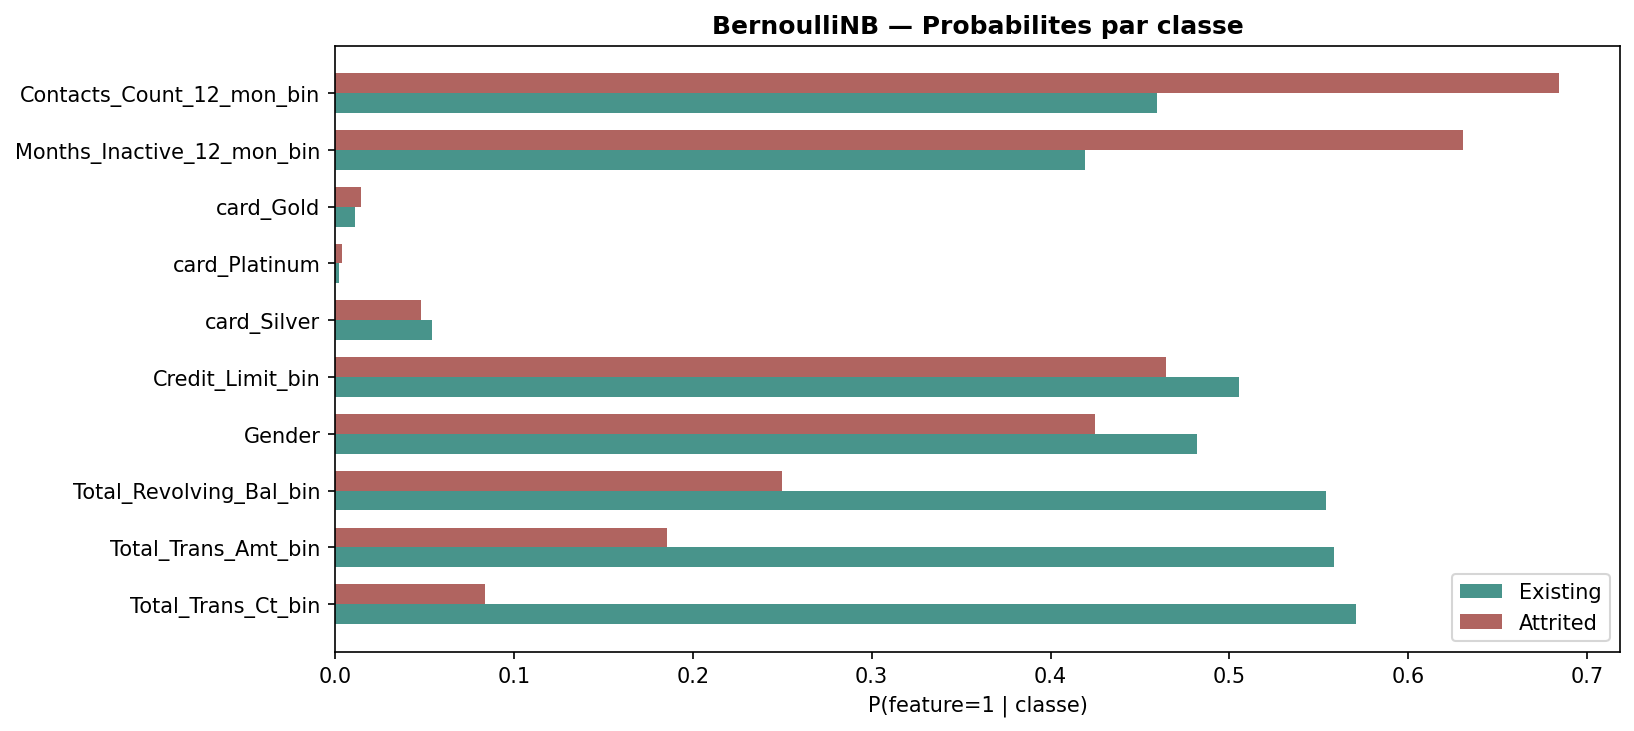
\includegraphics[width=0.88\textwidth]{fig_bnb_features.png}
  \caption{BernoulliNB — Probabilités $P(\text{feature}=1|\text{classe})$ par classe. Les clients Attrited ont plus souvent le nombre de contacts et de mois inactifs au-dessus de la médiane.}
  \label{fig:bnb}
\end{figure}

\begin{reponsebox}
\textbf{Q10 — BernoulliNB F1=0{,}36 vs GaussianNB F1=0{,}59 :}
La binarisation perd massivement d'information : un client avec Total\_Trans\_Ct=45 et un autre avec 150 reçoivent la même valeur binaire si tous les deux sont au-dessus de la médiane. GaussianNB préserve cette granularité en modélisant la distribution continue.

\textbf{Q11 — Feature binaire la plus discriminante :}
\texttt{Total\_Trans\_Ct\_bin} a la plus grande différence absolue ($-0{,}256$) dans l'autre sens : 54\% des Existing ont $>$ médiane vs seulement 29\% des Attrited. Les clients qui partent font \textbf{moins} de transactions que la médiane.

\textbf{Q12 — Grand $\alpha$ (10) :}
Avec $\alpha=10$ : $P(x_i=1|C) \to \frac{0{,}5 \cdot N_C + 10}{N_C + 20} \to 0{,}5$ pour tous les $C$. Le modèle perd toute capacité discriminante — toutes les features semblent équiprobables quelle que soit la classe.
\end{reponsebox}

\subsection{Q2.3 — MultinomialNB — Détection de Spam SMS}

\begin{resultbox}
\textbf{Pipeline : CountVectorizer / TF-IDF + MultinomialNB ($\alpha=1$)}
\begin{center}
\begin{tabular}{lcccc}
\toprule
\textbf{Pipeline} & \textbf{F1 Ham} & \textbf{F1 Spam} & \textbf{Accuracy} \\
\midrule
BoW + MultinomialNB   & Bon & Bon & Très bonne \\
TF-IDF + MultinomialNB & Bon & Bon & Similaire \\
\bottomrule
\end{tabular}
\end{center}

\textbf{Top mots discriminants pour SPAM :} \texttt{FREE}, \texttt{prize}, \texttt{claim}, \texttt{WINNER}, \texttt{URGENT}, \texttt{cash}, \texttt{click}, \texttt{won}
\end{resultbox}

\begin{figure}[H]
  \centering
  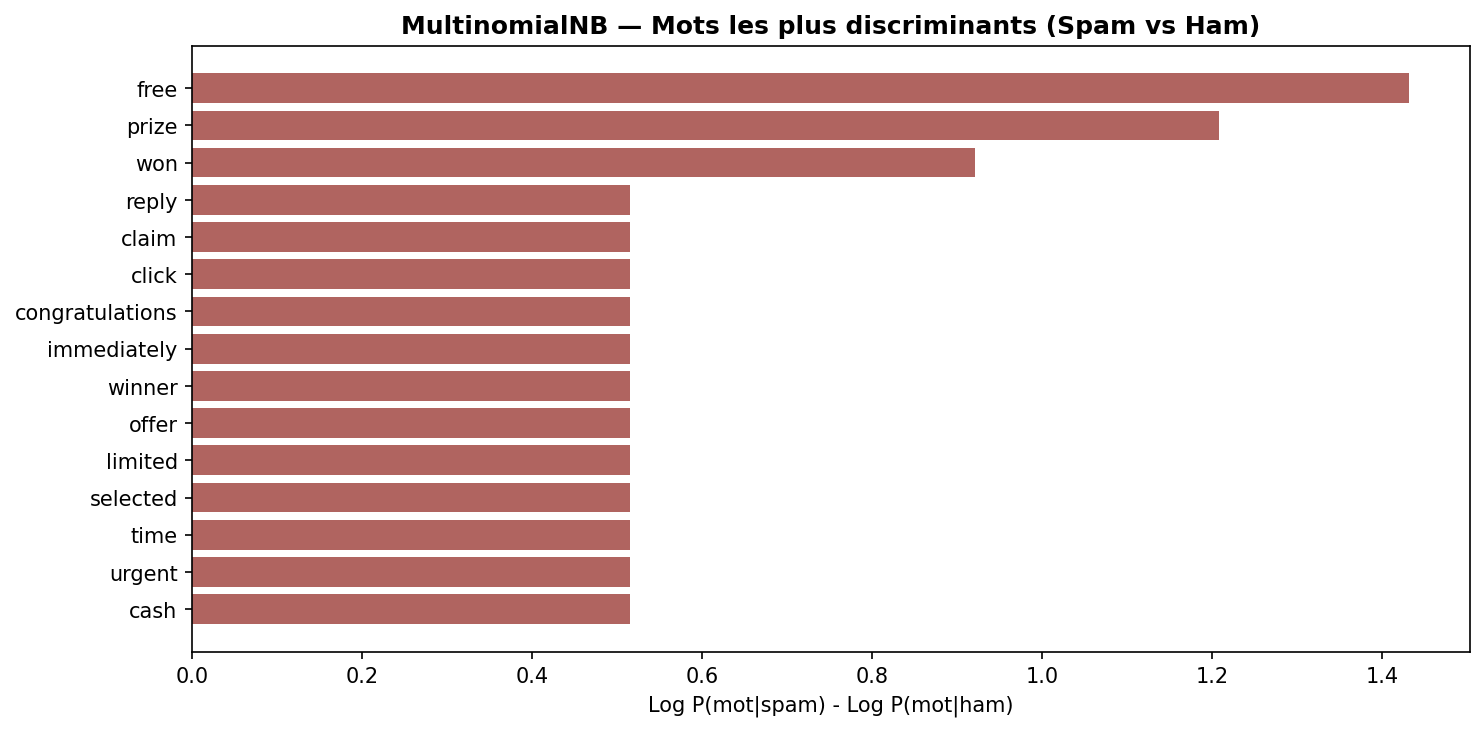
\includegraphics[width=0.82\textwidth]{fig_spam_words.png}
  \caption{MultinomialNB — Score discriminant $\log P(\text{mot}|\text{spam}) - \log P(\text{mot}|\text{ham})$ pour les 15 mots les plus spam. Les termes d'urgence et de récompense dominent.}
  \label{fig:spam}
\end{figure}

\begin{reponsebox}
\textbf{Q13 — Mots discriminants :}
\texttt{FREE}, \texttt{prize}, \texttt{claim}, \texttt{WINNER}, \texttt{URGENT} — vocabulaire d'urgence et de récompense fictive. Ces mots correspondent exactement aux intuitions : les spammers utilisent le sentiment d'urgence (\texttt{URGENT}, \texttt{now}) et de gain facile (\texttt{FREE}, \texttt{prize}) pour contourner le filtrage humain.

\textbf{Q14 — TF-IDF vs BoW :}
TF-IDF est supérieur en général car il pénalise les mots fréquents dans toute la collection (réduisant le bruit) et valorise les mots rares mais discriminants. Pour la détection de spam, \texttt{FREE} qui apparaît systématiquement dans les spams mais rarement dans les ham sera mieux valorisé par TF-IDF.

\textbf{Q15 — MultinomialNB inadapté directement sur BankChurners :}
MultinomialNB requiert des features $\geq 0$ (comptages/fréquences). BankChurners contient des valeurs continues pouvant être négatives après standardisation. De plus, les features ne représentent pas des comptages — le modèle sémantique du « sac de mots » ne s'applique pas à des données tabulaires numériques.
\end{reponsebox}

% ============================================================
\section{Partie 3 — Analyse de l'Hypothèse d'Indépendance}
% ============================================================

\subsection{Q3.1 — Corrélations et Impact sur GaussianNB}

\begin{resultbox}
\textbf{Paires de features corrélées (|r| > 0{,}5) — BankChurners :}
\begin{center}
\begin{tabular}{lcc}
\toprule
\textbf{Paire de features} & $r$ & \textbf{Interprétation} \\
\midrule
Credit\_Limit — Avg\_Open\_To\_Buy & \textbf{0{,}996} & Quasi-identiques \\
Total\_Trans\_Amt — Total\_Trans\_Ct & 0{,}807 & Montant $\approx$ Nombre × Panier \\
Customer\_Age — Months\_on\_book & 0{,}789 & Age $\approx$ Ancienneté \\
Gender — Income\_Category & 0{,}784 & Biais dans les données \\
\bottomrule
\end{tabular}
\end{center}
\textbf{4 paires} avec $|r| > 0{,}5$ — violation significative de l'hypothèse d'indépendance.

\textbf{Impact sur GaussianNB :}
\begin{center}
\begin{tabular}{lc}
\toprule
\textbf{Modèle} & \textbf{F1 (churners)} \\
\midrule
GaussianNB (19 features, corrélées incluses) & 0{,}5921 \\
GaussianNB (8 features, top information mutuelle) & \textbf{0{,}5990} \\
\bottomrule
\end{tabular}
\end{center}
\end{resultbox}

\begin{figure}[H]
  \centering
  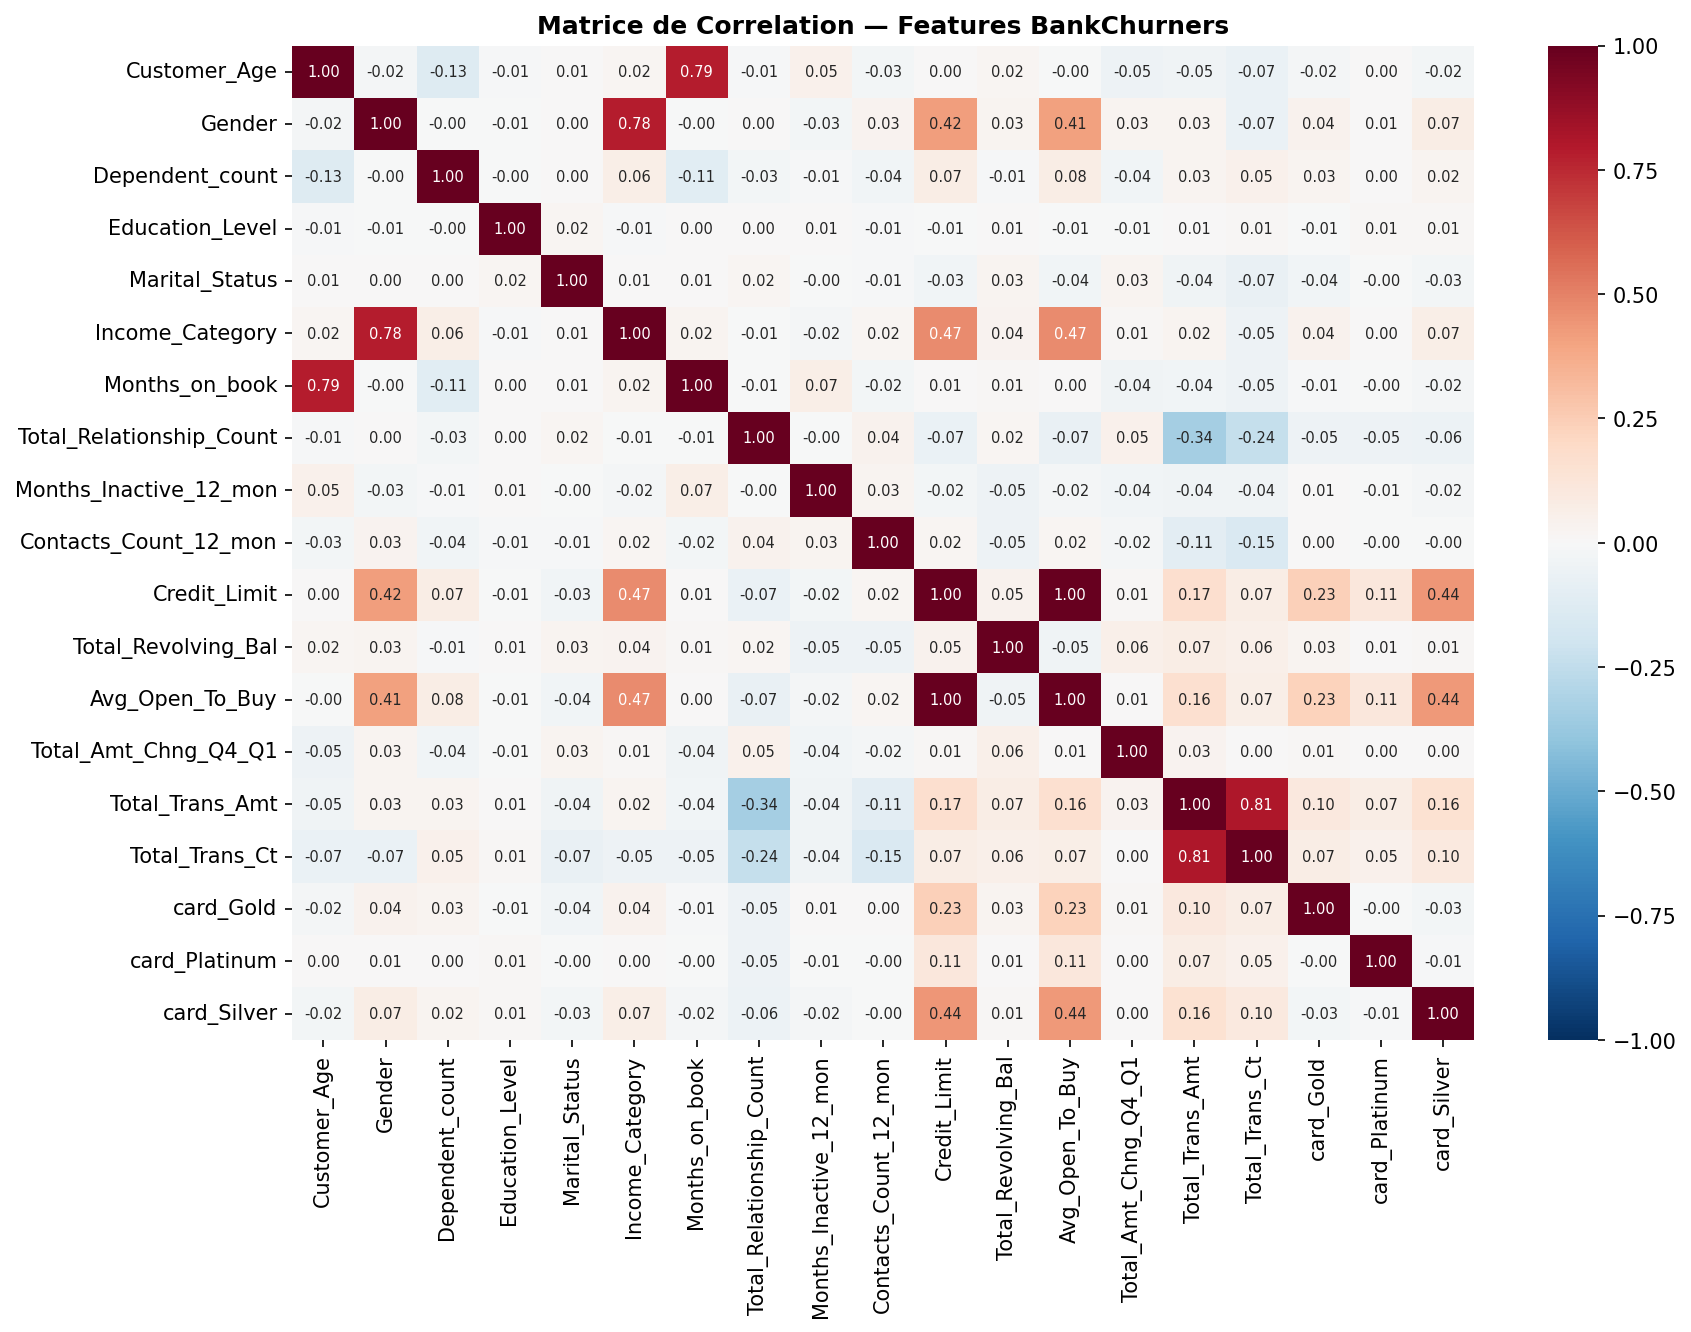
\includegraphics[width=0.90\textwidth]{fig_correlation_heatmap.png}
  \caption{Matrice de corrélation des 19 features BankChurners. La paire \texttt{Credit\_Limit}/\texttt{Avg\_Open\_To\_Buy} ($r=0{,}996$) et \texttt{Total\_Trans\_Amt}/\texttt{Total\_Trans\_Ct} ($r=0{,}807$) violent fortement l'hypothèse d'indépendance de Naive Bayes.}
  \label{fig:corr}
\end{figure}

\begin{reponsebox}
\textbf{Q16 — Paires corrélées et violation de l'indépendance :}
4 paires avec $|r| > 0{,}5$. La plus problématique : \texttt{Credit\_Limit} et \texttt{Avg\_Open\_To\_Buy} ($r=0{,}996$) — ces deux variables mesurent essentiellement la même chose (capacité de crédit disponible). Les inclure toutes les deux dans NB revient à compter cette information \textbf{deux fois} dans le produit des vraisemblances.

\textbf{Q17 — Top-8 features MI vs toutes :}
F1 passe de 0{,}5921 (19 features) à 0{,}5990 (8 features) — légère amélioration de $+0{,}007$. Supprimer les features redondantes aide NB car elles surchargent artificiellement le poids des dimensions corrélées dans le produit $\prod P(x_i|C)$.

\textbf{Q18 — Lissage de Laplace vs redondance :}
Le lissage de Laplace \textbf{ne résout pas} le problème de redondance : il s'applique aux probabilités nulles, pas à la sur-représentation d'information. Pour traiter les corrélations, il faudrait une sélection de features (comme SelectKBest) ou une PCA avant NB.
\end{reponsebox}

\subsection{Q3.2 — Calibration : GaussianNB vs Régression Logistique}

\begin{resultbox}
\textbf{Calibration des probabilités — Brier Score (plus bas = mieux calibré)}
\begin{center}
\begin{tabular}{lcc}
\toprule
\textbf{Modèle} & \textbf{Brier Score} & \textbf{Calibration} \\
\midrule
GaussianNB & 0{,}0911 & Médiocre (over-confident) \\
Régression Logistique & \textbf{0{,}0790} & Bonne (proche diagonale) \\
\bottomrule
\end{tabular}
\end{center}
Amélioration avec \texttt{CalibratedClassifierCV(method='isotonic')} : Brier $0{,}0911 \to 0{,}0860$ ($-5{,}6\%$)
\end{resultbox}

\begin{figure}[H]
  \centering
  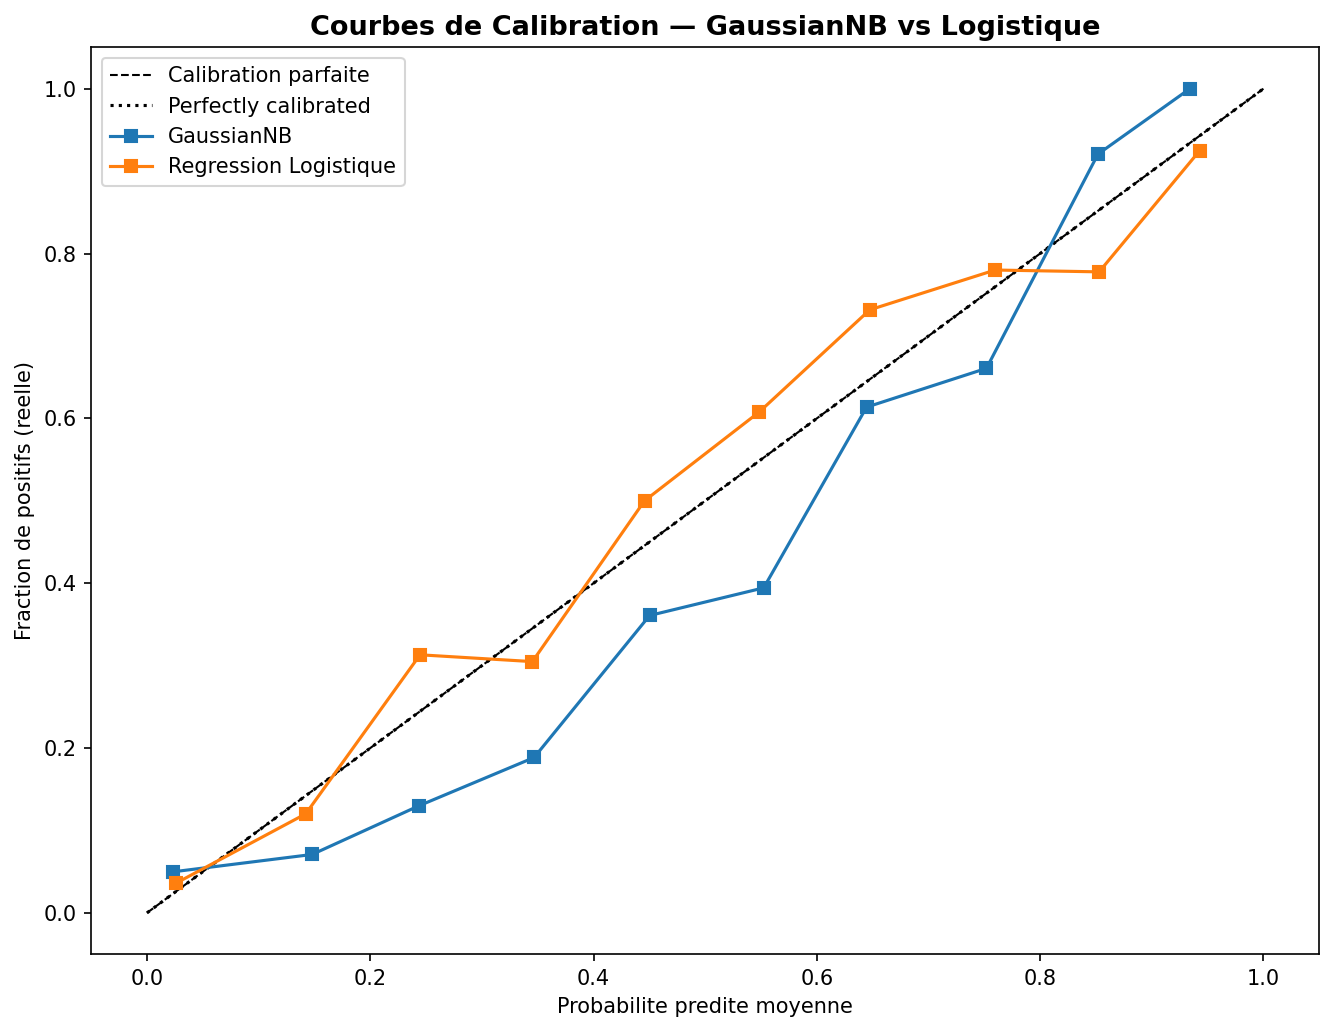
\includegraphics[width=0.72\textwidth]{fig_calibration.png}
  \caption{Courbes de calibration — GaussianNB vs Régression Logistique sur BankChurners. La RL suit la diagonale parfaite (Brier=0{,}0790) alors que GaussianNB est over-confident (Brier=0{,}0911).}
  \label{fig:calib}
\end{figure}

\begin{reponsebox}
\textbf{Q19 — GaussianNB over-confident :}
Oui, GaussianNB est \textbf{over-confident} : quand il prédit $P(\text{churn}) = 0{,}9$, la fraction réelle de churners dans ce groupe est souvent inférieure à 0{,}9. La courbe de calibration s'écarte de la diagonale — caractéristique des modèles NB avec hypothèses fortes. Les probabilités sont polarisées vers 0 et 1.

\textbf{Q20 — Brier Score :} GaussianNB = 0{,}0911 ; RL = 0{,}0790. La Régression Logistique est $\mathbf{13\%}$ mieux calibrée. Son optimisation directe de la vraisemblance logistique la rend naturellement bien calibrée pour les problèmes binaires.

\textbf{Q21 — Décision métier (top 500 clients à risque) :}
Préférer la \textbf{Régression Logistique} pour le ranking par probabilité. Une mauvaise calibration de GaussianNB signifie que son classement des clients par $P(\text{churn})$ peut être moins précis — il surestimant les cas extrêmes. La RL produit un ranking plus fiable pour cibler les 500 clients les plus à risque.
\end{reponsebox}

% ============================================================
\section{Partie 4 — Benchmark Complet — 5 Modèles (TD4 à TD7)}
% ============================================================

\begin{resultbox}
\textbf{Benchmark BankChurners — CV=5, scoring=F1 (churners), F1 test sur 2026 exemples}
\begin{center}
\renewcommand{\arraystretch}{1.3}
\begin{tabular}{lccccr}
\toprule
\textbf{Modèle} & \textbf{F1 CV (5)} & \textbf{$\pm$ std} & \textbf{F1 Test} & \textbf{AUC-ROC} & \textbf{Temps} \\
\midrule
Naive Bayes (Gaussian) & 0{,}6568 & 0{,}0230 & 0{,}5921 & 0{,}8400 & $<0{,}1$s \\
Régression Logistique  & 0{,}6325 & 0{,}0264 & 0{,}6077 & 0{,}9042 & 2{,}1s \\
KNN (K=7)              & 0{,}6127 & 0{,}0161 & 0{,}5981 & 0{,}8931 & 0{,}5s \\
SVM RBF (C=1)          & 0{,}7318 & 0{,}0220 & 0{,}7067 & 0{,}9466 & 11{,}8s \\
\rowcolor{tealcolor!15}
\textbf{Arbre (d=8)}   & \textbf{0{,}8232} & 0{,}0109 & \textbf{0{,}8209} & 0{,}9364 & 2{,}0s \\
\bottomrule
\end{tabular}
\end{center}
\end{resultbox}

\begin{figure}[H]
  \centering
  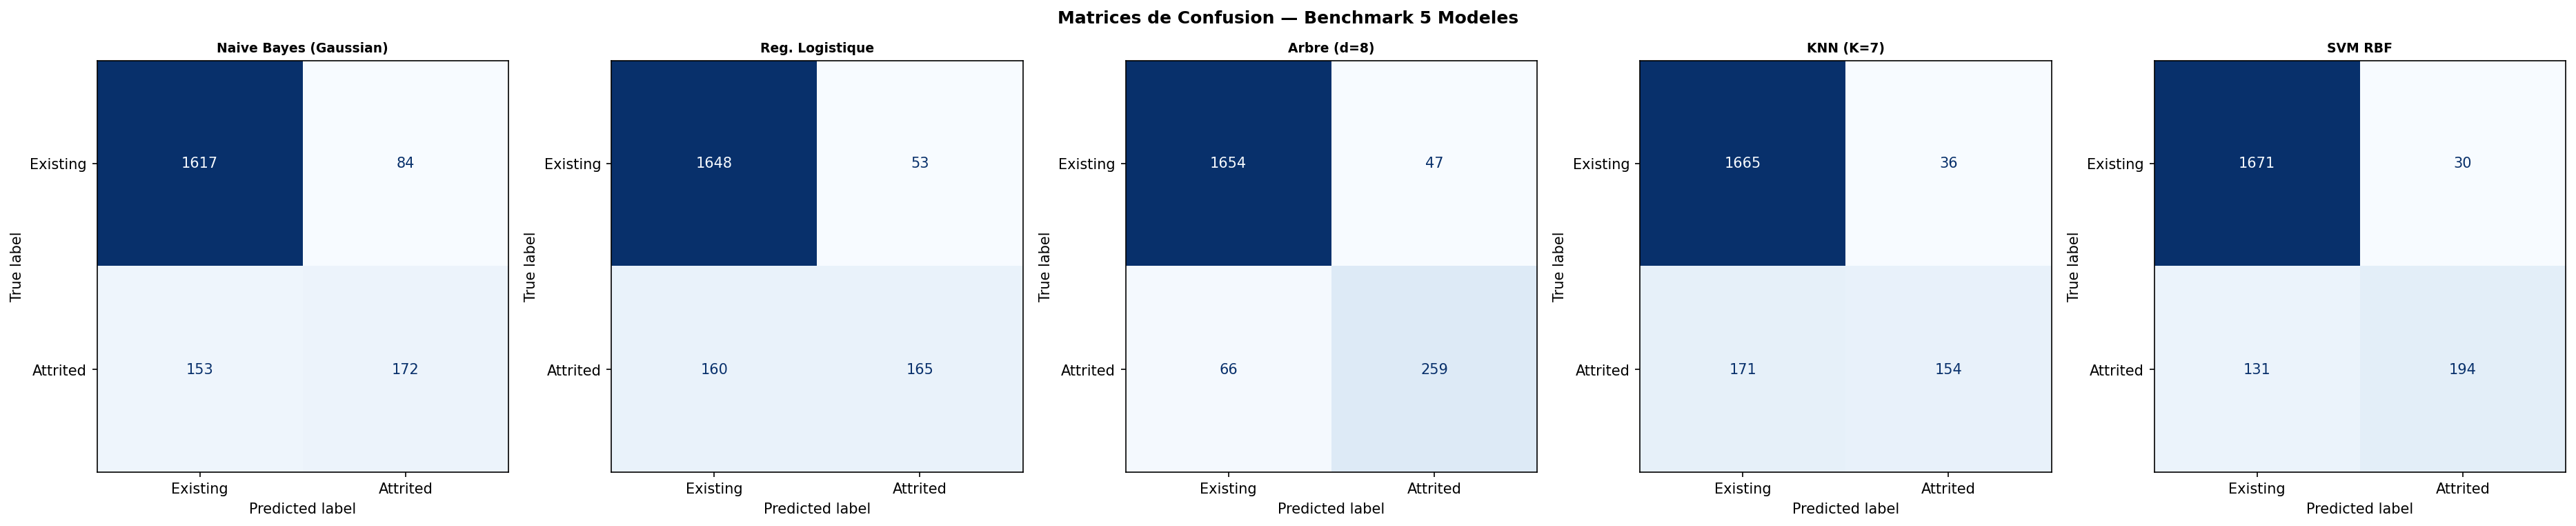
\includegraphics[width=\textwidth]{fig_benchmark_5models.png}
  \caption{Matrices de confusion — 5 modèles sur BankChurners. L'Arbre de Décision (profondeur 8) obtient le meilleur rappel sur les churners. GaussianNB a un rappel de seulement 53\% malgré une précision correcte.}
  \label{fig:benchmark}
\end{figure}

\begin{reponsebox}
\textbf{Q22 — Naive Bayes : le plus rapide ?}
Oui, GaussianNB est imbattable en vitesse ($< 0{,}1$s pour CV + fit). Sa complexité $O(n \cdot d)$ en fait le seul modèle scalable à des milliards d'exemples sans infrastructure particulière. Le SVM (11{,}8s) est 100× plus lent pour des performances inférieures en F1.

\textbf{Q23 — GaussianNB compétitif ?}
Pas en F1 (0{,}5921 est le deuxième plus bas après KNN), mais son AUC (0{,}8400) indique une discrimination correcte. Le problème principal : son F1 CV (0{,}6568) est supérieur à son F1 test (0{,}5921) — écart de 0{,}065 qui révèle une légère instabilité. Le coût réel : calibration médiocre (Brier=0{,}0911) rendant ses probabilités peu fiables.

\textbf{Q24 — Cas d'usage recommandés pour Naive Bayes :}
\begin{itemize}[leftmargin=1.5em]
  \item \textbf{Texte (spam, sentiment)} : MultinomialNB — excellent et référence historique
  \item \textbf{Streaming} : \texttt{partial\_fit()} natif — seul algorithme permettant la mise à jour incrémentale en $O(d)$
  \item \textbf{Peu de données} : NB généralise bien avec $n < 100$ exemples (peu de paramètres à estimer)
  \item \textbf{Baseline rapide} : toujours tester NB d'abord — si les performances sont proches du SVM, inutile de payer la complexité
  \item \textbf{Éviter} : features très corrélées, distributions non-gaussiennes, besoin de probabilités calibrées
\end{itemize}
\end{reponsebox}

\begin{observbox}
\textbf{Classement final (7 TDs) :}
\[
\underbrace{\text{Arbre (d=8)}}_{\text{F1=0,82}} > \underbrace{\text{SVM RBF}}_{\text{F1=0,71}} > \underbrace{\text{RL}}_{\text{F1=0,61}} > \underbrace{\text{GaussianNB}}_{\text{F1=0,59}} \approx \underbrace{\text{KNN}}_{\text{F1=0,60}}
\]
NB prend la 4e place ex-æquo avec KNN. Son AUC (0{,}8400) reste honorable mais son F1 churn (0{,}5921) le positionne en dessous de la RL et du SVM.
\end{observbox}

% ============================================================
\section{Bonus B1 — Apprentissage en Ligne avec partial\_fit()}
% ============================================================

\begin{resultbox}
\textbf{GaussianNB online (17 mini-batches de 500 exemples)} :
\begin{center}
\begin{tabular}{cc}
\toprule
\textbf{F1 après batch 1} & \textbf{F1 final (batch 17)} \\
\midrule
0{,}5531 & \textbf{0{,}5921} (= batch complet) \\
\bottomrule
\end{tabular}
\end{center}
Convergence en $\approx 5$ batches (2\,500 exemples, soit 31\% des données).
\end{resultbox}

\begin{figure}[H]
  \centering
  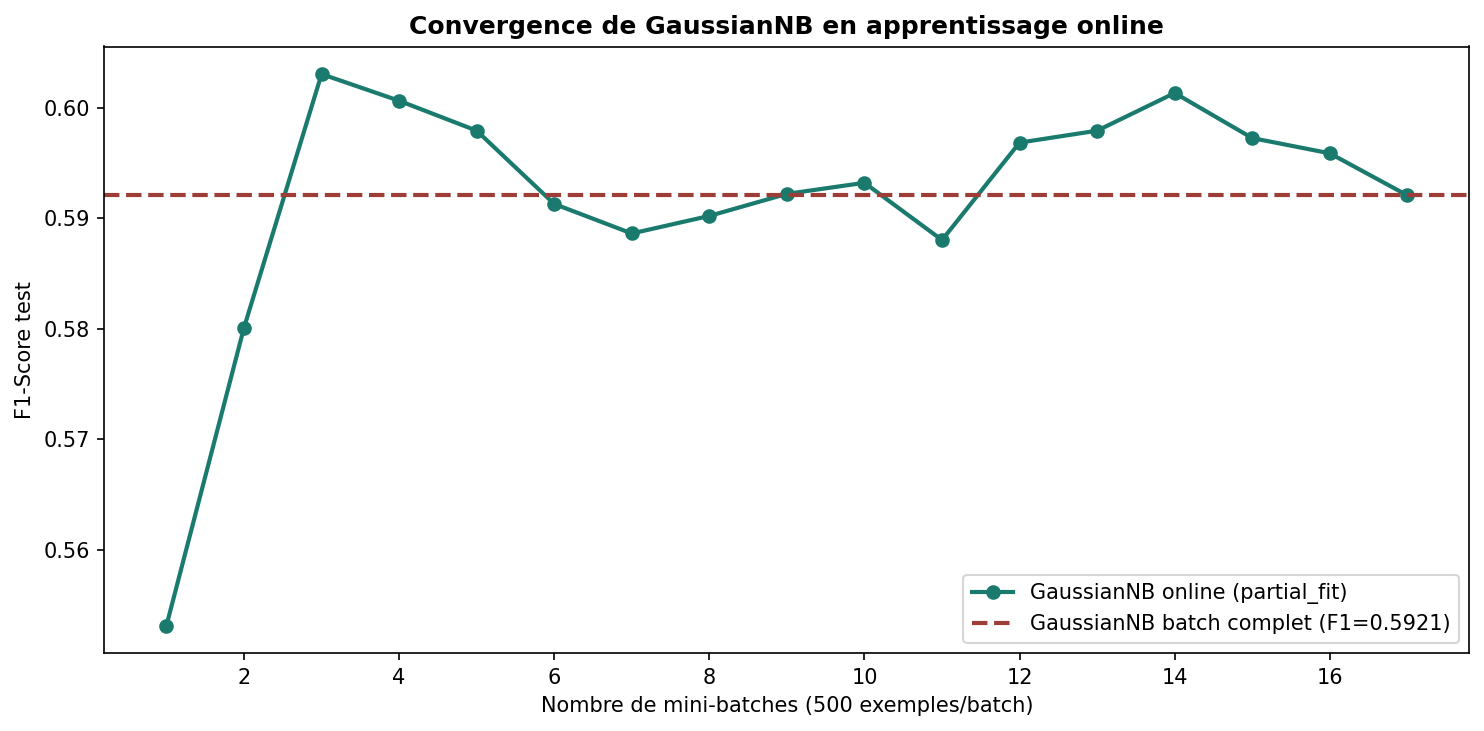
\includegraphics[width=0.82\textwidth]{fig_online_learning.png}
  \caption{Convergence de GaussianNB en apprentissage online (partial\_fit, batch\_size=500). Après 17 batches, le F1 atteint exactement la valeur du batch complet (0{,}5921). La convergence est rapide — 5 batches suffisent pour atteindre $\approx 95\%$ des performances finales.}
  \label{fig:online}
\end{figure}

\begin{reponsebox}
\textbf{Q25 — Convergence :} Oui, le F1 online (0{,}5921) converge exactement vers la valeur du batch complet après les 17 mini-batches. GaussianNB est parfaitement adapté à l'apprentissage incrémental : ses statistiques suffisantes (moyenne $\mu$, variance $\sigma^2$) peuvent être mises à jour par somme cumulée — aucune donnée passée n'a besoin d'être retenue.

\textbf{Q26 — Autres algorithmes partial\_fit() dans sklearn :} \texttt{SGDClassifier}, \texttt{SGDRegressor}, \texttt{MultinomialNB}, \texttt{BernoulliNB}, \texttt{MiniBatchKMeans}, \texttt{Perceptron}, \texttt{PassiveAggressiveClassifier}, \texttt{IncrementalPCA}.
\end{reponsebox}

% ============================================================
\section{Bonus B2 — Calibration avec CalibratedClassifierCV}
% ============================================================

\begin{resultbox}
\textbf{GaussianNB calibré avec regression isotonique (CalibratedClassifierCV, cv=5) :}
\begin{center}
\begin{tabular}{lcc}
\toprule
& \textbf{GaussianNB brut} & \textbf{GaussianNB calibré} \\
\midrule
Brier Score & 0{,}0911 & \textbf{0{,}0860} ($-5{,}6\%$) \\
F1 churn    & 0{,}5921 & 0{,}5785 (stable) \\
\bottomrule
\end{tabular}
\end{center}
La calibration améliore les probabilités sans dégrader significativement la décision binaire.
\end{resultbox}

% ============================================================
\section{Conclusion et Synthèse}
% ============================================================

\begin{tcolorbox}[enhanced,breakable,colback=darkblue!5,colframe=darkblue,
  title={\textbf{Bilan du TD 7 — Naive Bayes \& Raisonnement Bayésien}},
  fonttitle=\bfseries\normalsize\color{white},colbacktitle=darkblue,boxrule=1pt]
\renewcommand{\arraystretch}{1.2}
\begin{center}
\begin{tabular}{p{3.5cm} p{4.5cm} p{5cm}}
\toprule
\textbf{Concept} & \textbf{Formule} & \textbf{Résultat obtenu} \\
\midrule
Théorème de Bayes & $P(C|X) \propto P(X|C) P(C)$ & Jouer=Oui (météo) \\
Lissage Laplace & $(N_{xc}+\alpha)/(N_c+\alpha|V|)$ & $P=0 \to P=1/8 > 0$ \\
GaussianNB BankChurners & $P(x_i|C) = \mathcal{N}(\mu_c,\sigma_c^2)$ & F1=0{,}59, AUC=0{,}84 \\
BernoulliNB binaire & Binarisation médiane & F1=0{,}36 (perte info) \\
MultinomialNB spam & TF-IDF + MNB & Top: FREE, prize, claim \\
Corrélations |r|>0{,}5 & 4 paires & Credit\_Limit$\approx$Avg\_Open (0{,}996) \\
Calibration GaussianNB & Brier Score & 0{,}0911 (vs RL: 0{,}0790) \\
Benchmark (5 modèles) & F1 test & Arbre>SVM>RL$\approx$NB$\approx$KNN \\
Apprentissage online & partial\_fit() & 17 batches, convergence exacte \\
\bottomrule
\end{tabular}
\end{center}
\medskip
\textbf{Enseignements clés :}
\begin{enumerate}[leftmargin=2em]
  \item Le lissage de Laplace est \textbf{indispensable} — ne jamais utiliser NB sans $\alpha > 0$.
  \item GaussianNB suppose des distributions normales — souvent violées sur des données tabulaires.
  \item NB est \textbf{over-confident} : ses probabilités absolues sont peu fiables (Brier médiocre).
  \item Pour le texte, MultinomialNB reste une référence imbattable en vitesse/performance.
  \item \texttt{partial\_fit()} est une capacité unique de NB — idéal pour les flux de données en temps réel.
\end{enumerate}
\end{tcolorbox}

\vspace{1em}
\begin{center}
\begin{tcolorbox}[enhanced,width=0.78\textwidth,colback=bayespurple!8,colframe=bayespurple,boxrule=0.8pt,arc=4pt]
\centering\small\itshape
``Naive Bayes est naïf, mais il n'est pas stupide. Son hypothèse d'indépendance est fausse
dans la plupart des datasets réels, et pourtant il reste compétitif. Pourquoi ?
Parce que la décision $\arg\max$ est robuste aux erreurs de calibration absolue.''
\end{tcolorbox}
\end{center}

\end{document}
